\section{Зависимости показателя преломления и коэффициента поглощения от частоты. Дисперсионная формула Зелмеера. Фазовая и групповая скорости. Формула Рэлея.}
\subsection{Зависимости показателя преломления и коэффициента поглощения от частоты}
На некоторых экспериментах люди стали замечать зависимость показателя преломления от длины волны(частоты) падающего света, знаменитое разделение пучка посредством призмы:
\begin{figure}[h]\label{qr}
	\center{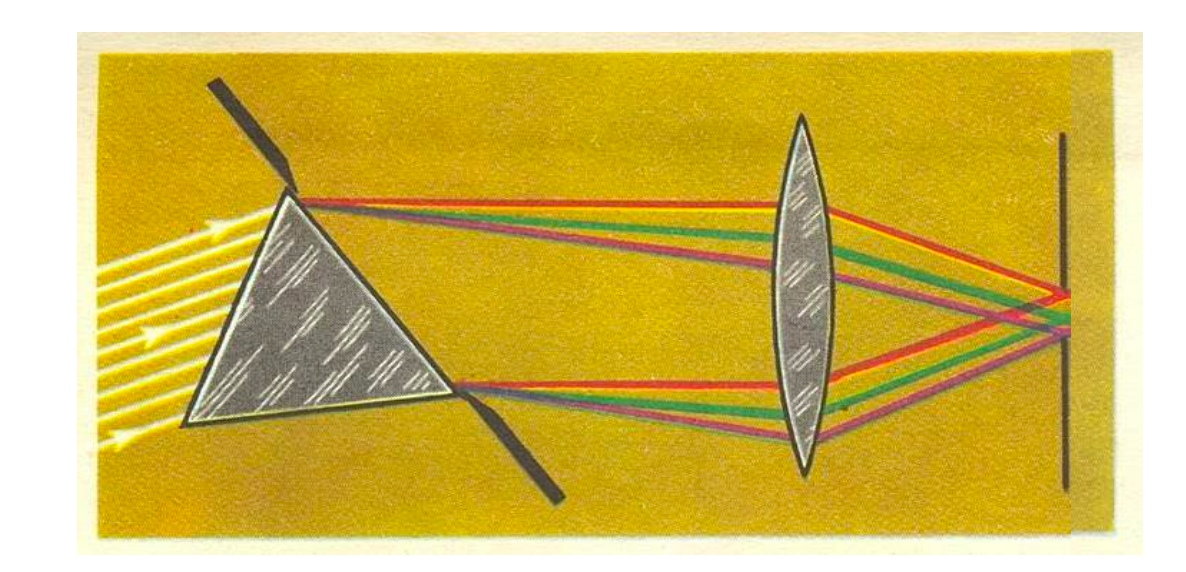
\includegraphics[scale=0.25]{41_1.jpg}}
	\caption{Иллюстрация дисперсии}
	\label{fig:image}
\end{figure}


Первая формула, которая описывала это называется \textbf{формулой Коши}(нормальный ход дисперсии), она представляет рял по обратным четным степеням длины волны:
\begin{equation}
n(\lambda) = a + b/\lambda^2 + c/\lambda^4 + ...
\end{equation}
Эта формула абсолютно эмпирическая и поэтому числовые коэффициенты должны быть найдены в ходе эксперимента.

Дальше про микроскопическую теорию: запишем показатель преломления через диэлектрическую проницаемость: $n = \sqrt{\varepsilon}$, также поговорим о специфике задачи: атом в электрическом поле это диполь с дипольным моментом равным : $p = r\cdot e$. Тогда запишем уравнение движения атомного осциллятора:
\begin{equation}
m \ddot{r} = eE - kr - \gamma \dot{r}
\end{equation}
где второе слагаемое определяет удерживающую силу, а третье диссипацию энергии. Немного преобразовав (заменив радиус вектор на дипольный момент, а также умножив на e/m ) получим: 
\begin{equation}
p + \gamma \dot{p} + \omega_{0}^2 p = \frac{e^2}{m}E_0 e^{-i\omega t}
\end{equation}
Где расписана плоская волна, и в ней мы считаем, что заряд локализован в окрестности начала координат, а также скорость приобретаемая при колебаниях значительно меньше скорости света, поэтому действием магнитного поля можно пренебречь. Такое уравнение решается экспоненциальным анзацем, поэтому решение имеет вид:
\begin{equation}
p=\frac{e^{2} E_{0}}{m} \cdot \frac{1}{\left(\omega_{0}^{2}-\omega^{2}\right)-(i \gamma \omega)} e^{-i \omega t}
\end{equation}
Дальше вспомним определение тела --- это среда состоящая из диполей, а поэтому мы зная некоторые соотношения между основными электромагнитными характеристиками получить :
\begin{equation}
D = E + 4 \pi P = E + 4 \pi N p = \varepsilon E
\end{equation}
Откуда несложно выражается диэлектрическая проницаемость:
\begin{equation}\label{eps}
\varepsilon=1+\frac{4 \pi N e^{2}}{m} \cdot \frac{1}{\left(\omega_{0}^{2}-\omega^{2}\right)-i \gamma \omega}
\end{equation}
Вспоминаем, что показатель преломления --- это корень из эпсилон, а поэтому становиться понятно, что во--первых легитимно существование мнимого показателя преломления, а во--вторых, вследствие многозначности корня мы получаем много ветвей нашего показателя преломления.


Также можно без труда заметить, что имеется резонансный характер, а значит без трения и в ситуации совпадения внешней и внутренней частот будет наблюдаться резонанс.

Теперь распишем показатель преломления: $\hat{n} = n(1-i\varkappa)$, где $\varkappa$ -- коэффициент поглощения. а дальше используя выражение \eqref{eps} получим два выражения, определяющие зависимости из названия главы: 
\begin{equation}
n^{2}\left(1-\varkappa^{2}\right)=1+4 \pi \frac{e}{m} N_{0} \frac{f\left(\omega_{0}^{2}-\omega^{2}\right)}{\left(\omega_{0}^{2}-\omega^{2}\right)^{2}+\omega^{2}(\gamma / m)^{2}}
\end{equation}
\begin{equation}
2 n^{2} \varkappa=4 \pi \frac{e}{m} N_{0} \frac{f(\gamma / m) \omega}{\left(\omega_{0}^{2}-\omega^{2}\right)+\omega^{2}(\gamma / m)^{2}}
\end{equation}
где первое кривая дисперсии, а вторая кривая поглощения (абсорбции): 
\begin{figure}[h]\label{qr}
	\center{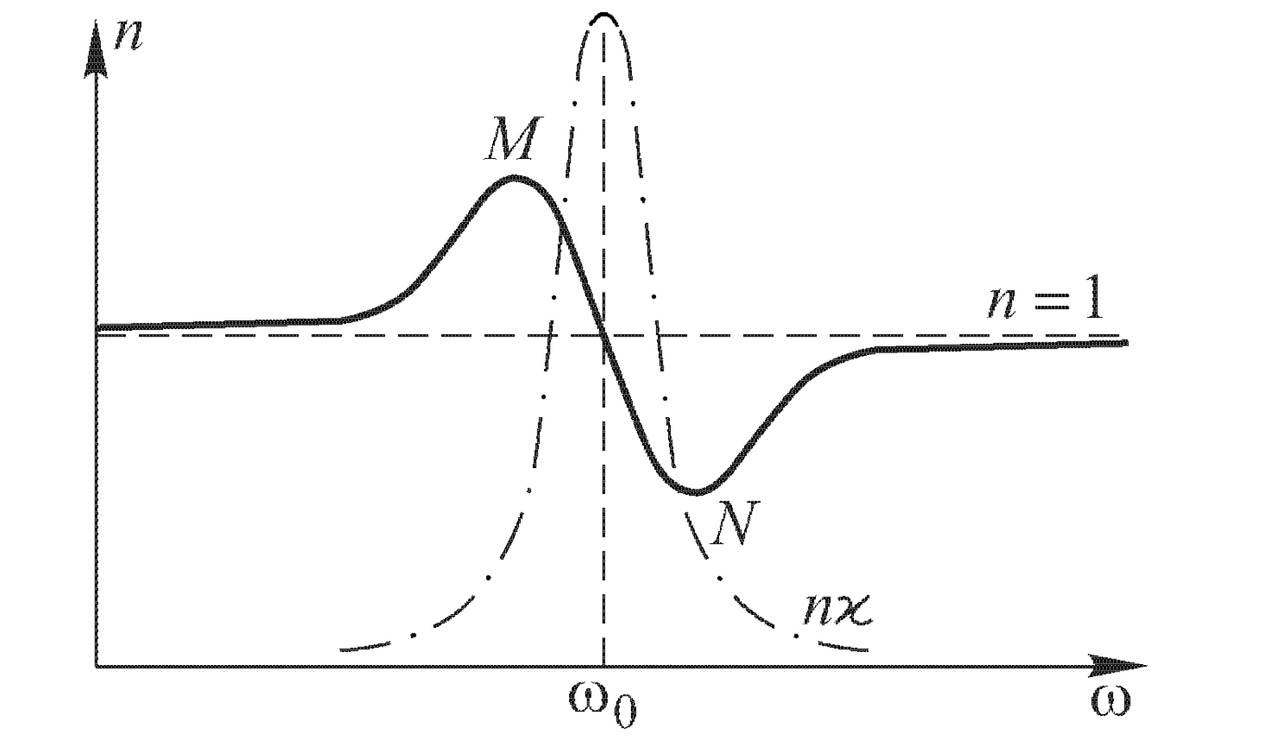
\includegraphics[scale=0.25]{41_2.jpg}}
	\caption{ Кривая дисперсии (сплошная) и абсорбции (пунктирная)}
	\label{fig:image}
\end{figure}


Если также учесть взаимодействие с молекула среды(вот так $E^{\prime}=E+\frac{4 \pi}{3} P$) получаем формулу Лоренц - Лорентца:
\begin{equation}
\frac{n^{2}-1}{n^{2}+1}=N_{0} \frac{4 \pi e^{2} f}{3 m\left(\omega_{0}^{2}-\omega^{2}\right)}
\end{equation}

\subsection{Дисперсионная формула Зельмейера}

Если полос поглощения(резонансов) много, тогда мы получаем (пренебрегая затуханием) и суммируем по всем частотам переходов получаем:
\begin{equation}
n^{2}=1+4 \pi N_{0} \sum \frac{f_{i} e_{i}^{2}}{m_{i}} \frac{1}{\left(\omega_{0 i}^{2}-\omega^{2}\right)}
\end{equation}
Где через $f_i$-- обозначена сила.
\begin{figure}[h]\label{qr}
	\center{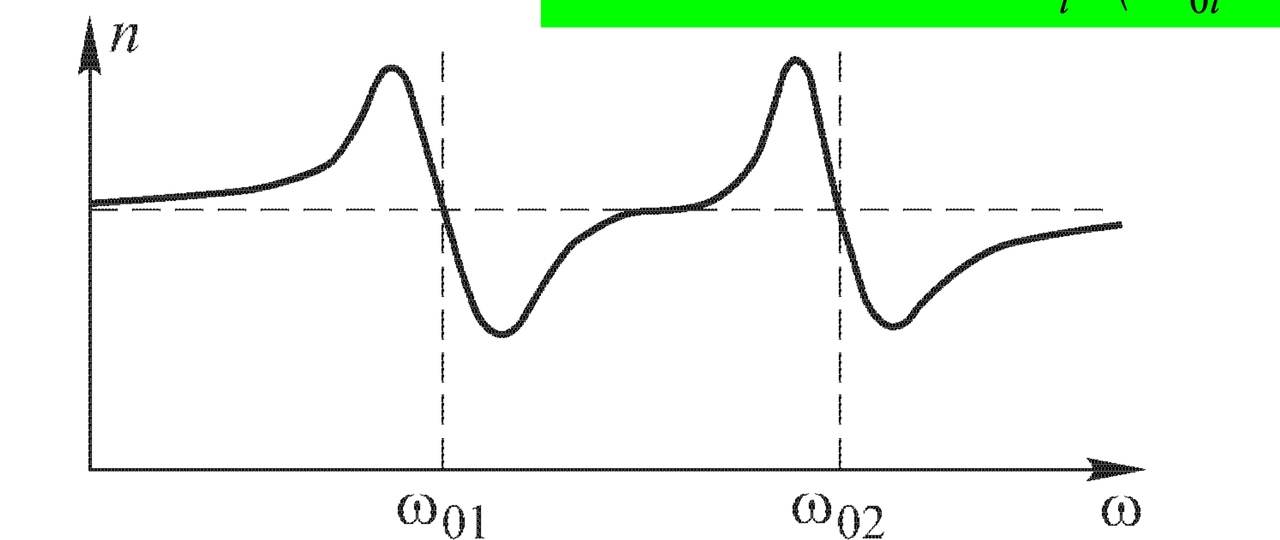
\includegraphics[scale=0.25]{41_3.jpg}}
	\caption{ Кривая дисперсии при нескольких резонансах}
	\label{fig:image}
\end{figure}
\subsection{Фазовая и групповая скорость, формула Рэлея}
\Def{Фазовая скорость} --- скорость распространения волнового фронта: $V = \omega/k=c/n$, в вакууме совпадает со скоростью света.

Теперь попробуем осознать, что такое групповая скорость: рассмотрим движения волнового пакета с шириной частот $2\delta \omega \ll \omega_0$, распишем два закона движения волн, для двух крайних частот спектра: 
\begin{equation}
y_{1}=a \sin \left(\omega_{1} t-k_{1} x\right) \quad \text { и } \quad y_{2}=a \sin \left(\omega_{2} t-k_{2} x\right), \quad \omega_{1,2}= \omega_0 \pm \delta \omega
\end{equation}

Просуммируем и преобразуем тригонометрическими формулами:

\begin{equation}
y=y_{1}+y_{2}=\underbrace{2 a \cos (t \delta \omega-x \delta k)}_{A} \sin \left(\omega_{0} t-k_{0} x\right)
\end{equation}
Выделим на импульсе точку, где $\boldsymbol{A}$ максимально. Скорость перемещения этой
точки характеризует скорость распространения импульса. Таким образом,
скорость импульса (группы), которую, по Рэлею, называют \Def{групповой
скоростью}, есть скорость перемещения амплитуды, $a,$ следовательно
энергии, переносимой движущимся импульсом.
\begin{equation}
A=\text {const} \Rightarrow t \delta \omega-x \delta k=\text {const} \Rightarrow \delta \omega d t-\delta k d x=0
\end{equation}
Отсюда найдем, что групповая скорость равна: 
\begin{equation}
u = \frac{dx}{dt} = \frac{\delta \omega}{\delta k} = \frac{d\omega}{dk}
\end{equation}
Выразив фазовую скорость через волновой вектор и используя определение длины волны, несложно получить \Def{формулу Рэлея}:
\begin{equation}
u=\frac{d \omega}{d k}=\frac{d(V k)}{d k}=V+k \frac{d V}{d k}, k=\frac{2 \pi}{\lambda}
\end{equation}
\begin{equation}
\fbox{$u=V-\lambda \dfrac{d V}{d \lambda}$}
\end{equation}
Можно немного преобразовать и получить:
\begin{equation}
u=\frac{c}{n+\omega \cdot d n / d \omega}
\end{equation}


Если говорить о геометрическом смысле фазовой и групповой скорости нетрудно получить, что 
\begin{figure}[h]\label{qr}
	\center{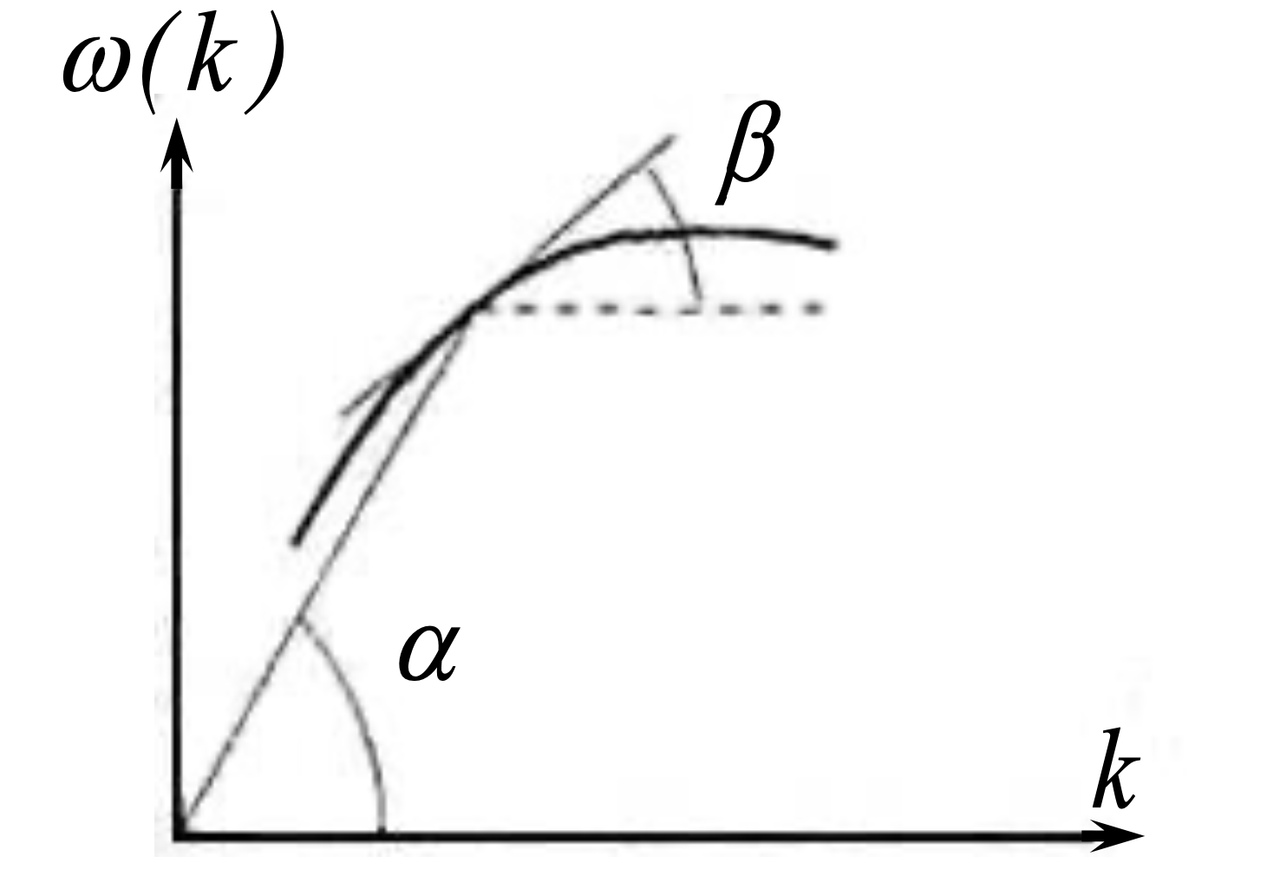
\includegraphics[scale=0.25]{41_4.jpg}}
	\caption{ $\tan\alpha$ --- фазовая скорость, $\tan\beta$ --- групповая скорость}
	\label{fig:image}
\end{figure}
